% When the farmer learns the yields: the three information structures of Lecture 10
% (Stochastic Programming: Information and Risk), sections II-III.
%
% Single source for the diagram in
%   optimization-private/lecture-notes/lectures/stochastic-programming-advanced.tex
% which \input's this file via \figsrc. Rendered to ../media/figures/sp-information-timing.{png,svg}
% by `make ../media/figures/sp-information-timing.png ../media/figures/sp-information-timing.svg`.
%
% Content is the lecture's own (no new claims): WS chooses everything after the yields are
% revealed (Birge & Louveaux 4.1, (1.2)); RP chooses acreage x first, then trades
% (B&L 4.1, (1.3)); EEV fixes x = x_EV from the mean-yield problem, then trades (B&L 4.2, (2.2)).
%
% Greyscale: black and grey line art only (house precedent, see decision-loop.tex). A decision
% is a SOLID box; the moment the yields are revealed is a DASHED grey box with an italic label,
% so the line style and the text each carry the distinction on their own.

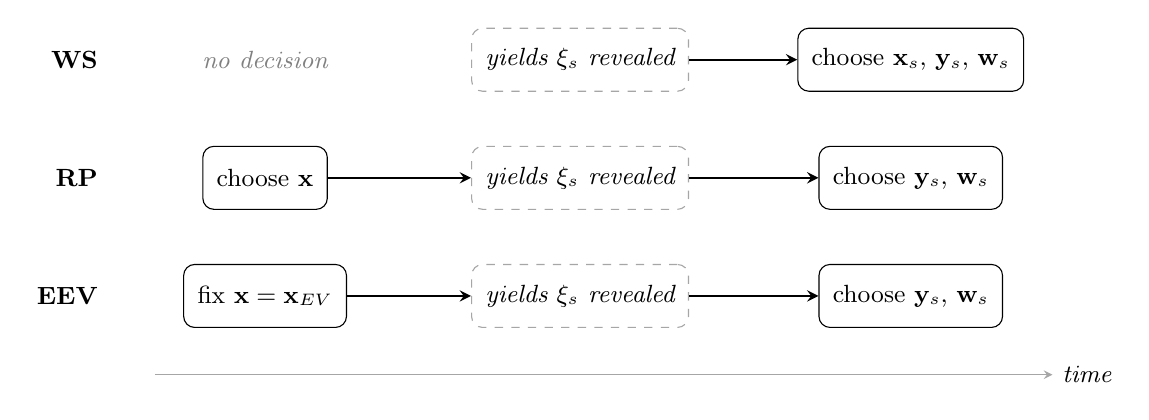
\begin{tikzpicture}[>=stealth,
    dec/.style={draw=black, fill=white, rounded corners, minimum height=8mm,
                inner xsep=5pt, font=\small, align=center},
    nat/.style={draw=gray!70, dashed, fill=white, rounded corners, minimum height=8mm,
                inner xsep=5pt, font=\small\itshape, align=center},
    flow/.style={->, thick, draw=black},
    lab/.style={font=\small\bfseries, anchor=east, align=right}]

  % ---- WS: yields first, then every decision
  % Columns: before the yields (x = 1.6), the revelation (x = 5.6), after (x = 9.8).
  \node[lab] at (-0.4,0) {WS};
  \node[font=\small\itshape, text=gray] at (1.6,0) {no decision};
  \node[nat] (w1) at (5.6,0)  {yields $\boldsymbol{\xi}_s$ revealed};
  \node[dec] (w2) at (9.8,0)  {choose $\mathbf{x}_s$, $\mathbf{y}_s$, $\mathbf{w}_s$};
  \draw[flow] (w1) -- (w2);

  % ---- RP: acreage, then yields, then trades
  \node[lab] at (-0.4,-1.5) {RP};
  \node[dec] (r1) at (1.6,-1.5)  {choose $\mathbf{x}$};
  \node[nat] (r2) at (5.6,-1.5)  {yields $\boldsymbol{\xi}_s$ revealed};
  \node[dec] (r3) at (9.8,-1.5)  {choose $\mathbf{y}_s$, $\mathbf{w}_s$};
  \draw[flow] (r1) -- (r2);
  \draw[flow] (r2) -- (r3);

  % ---- EEV: the mean-yield acreage, then yields, then trades
  \node[lab] at (-0.4,-3.0) {EEV};
  \node[dec] (e1) at (1.6,-3.0)  {fix $\mathbf{x}=\mathbf{x}_{EV}$};
  \node[nat] (e2) at (5.6,-3.0)  {yields $\boldsymbol{\xi}_s$ revealed};
  \node[dec] (e3) at (9.8,-3.0)  {choose $\mathbf{y}_s$, $\mathbf{w}_s$};
  \draw[flow] (e1) -- (e2);
  \draw[flow] (e2) -- (e3);

  % ---- time axis
  \draw[->, gray!70] (0.2,-4.0) -- (11.6,-4.0)
    node[right, font=\small\itshape, text=black] {time};
\end{tikzpicture}
